\cvevent{\printinfo{\faPlusSquare}{스마트팩토리 IIoT PdM 플랫폼 개발}}{(주)아프로스 개발참여: 100\%}{2018.03 -- 2019}{Seoul, Korea}

\begin{itemize}[label=\emoji{satellite}]
	\item 소개: 스마트팩토리 IIoT PdM 솔루션 개발
	\item 참여 개발 내용: Edge Device(DAQ/Analysis) 애플리케이션 개발, 웹플랫폼 개발
	\item 개발 스택 및 프레임워크: *nix, NodeJS N-API, C++, golang, Python, Redis, MongoDB, GraphQL, ReactJS
	\item 참여 개발 내용
	      \begin{itemize}[label=\emoji{pushpin}]
		      \item 데이터 분석: Diagnosis(HMB-SD 기법 적용, Deep analyzed features), Prognosis(유사성기반 RUL 추정기법)
		      \item Anomaly detection, Disgnosis, Prognosis, Transient event 분류 데이터 누적
		      \item MQTT 브로커, Kafka 분산 메시지 큐, DB구축, GraphQL API 구축
		      \item 디바이스 관리 클라이언트, 플랫폼 클라이언트 개발 (ReactJS)
	      \end{itemize}
	\item 개발 스택 및 프레임워크: JavaScript(ES6), Babel, NodeJS, C++, golang, GraphQL, ReactJS, ElectronJS, Python
	\item 현장 테스트베드 가동: SK하이닉스, SK텔레콤, KETI, 남강정밀등. 80여개소 디플로이 및 유지관리
\end{itemize}
\begin{figure}[!ht]
	\begin{fullwidth}
		\parbox{0.5\textwidth}{
			\centering
			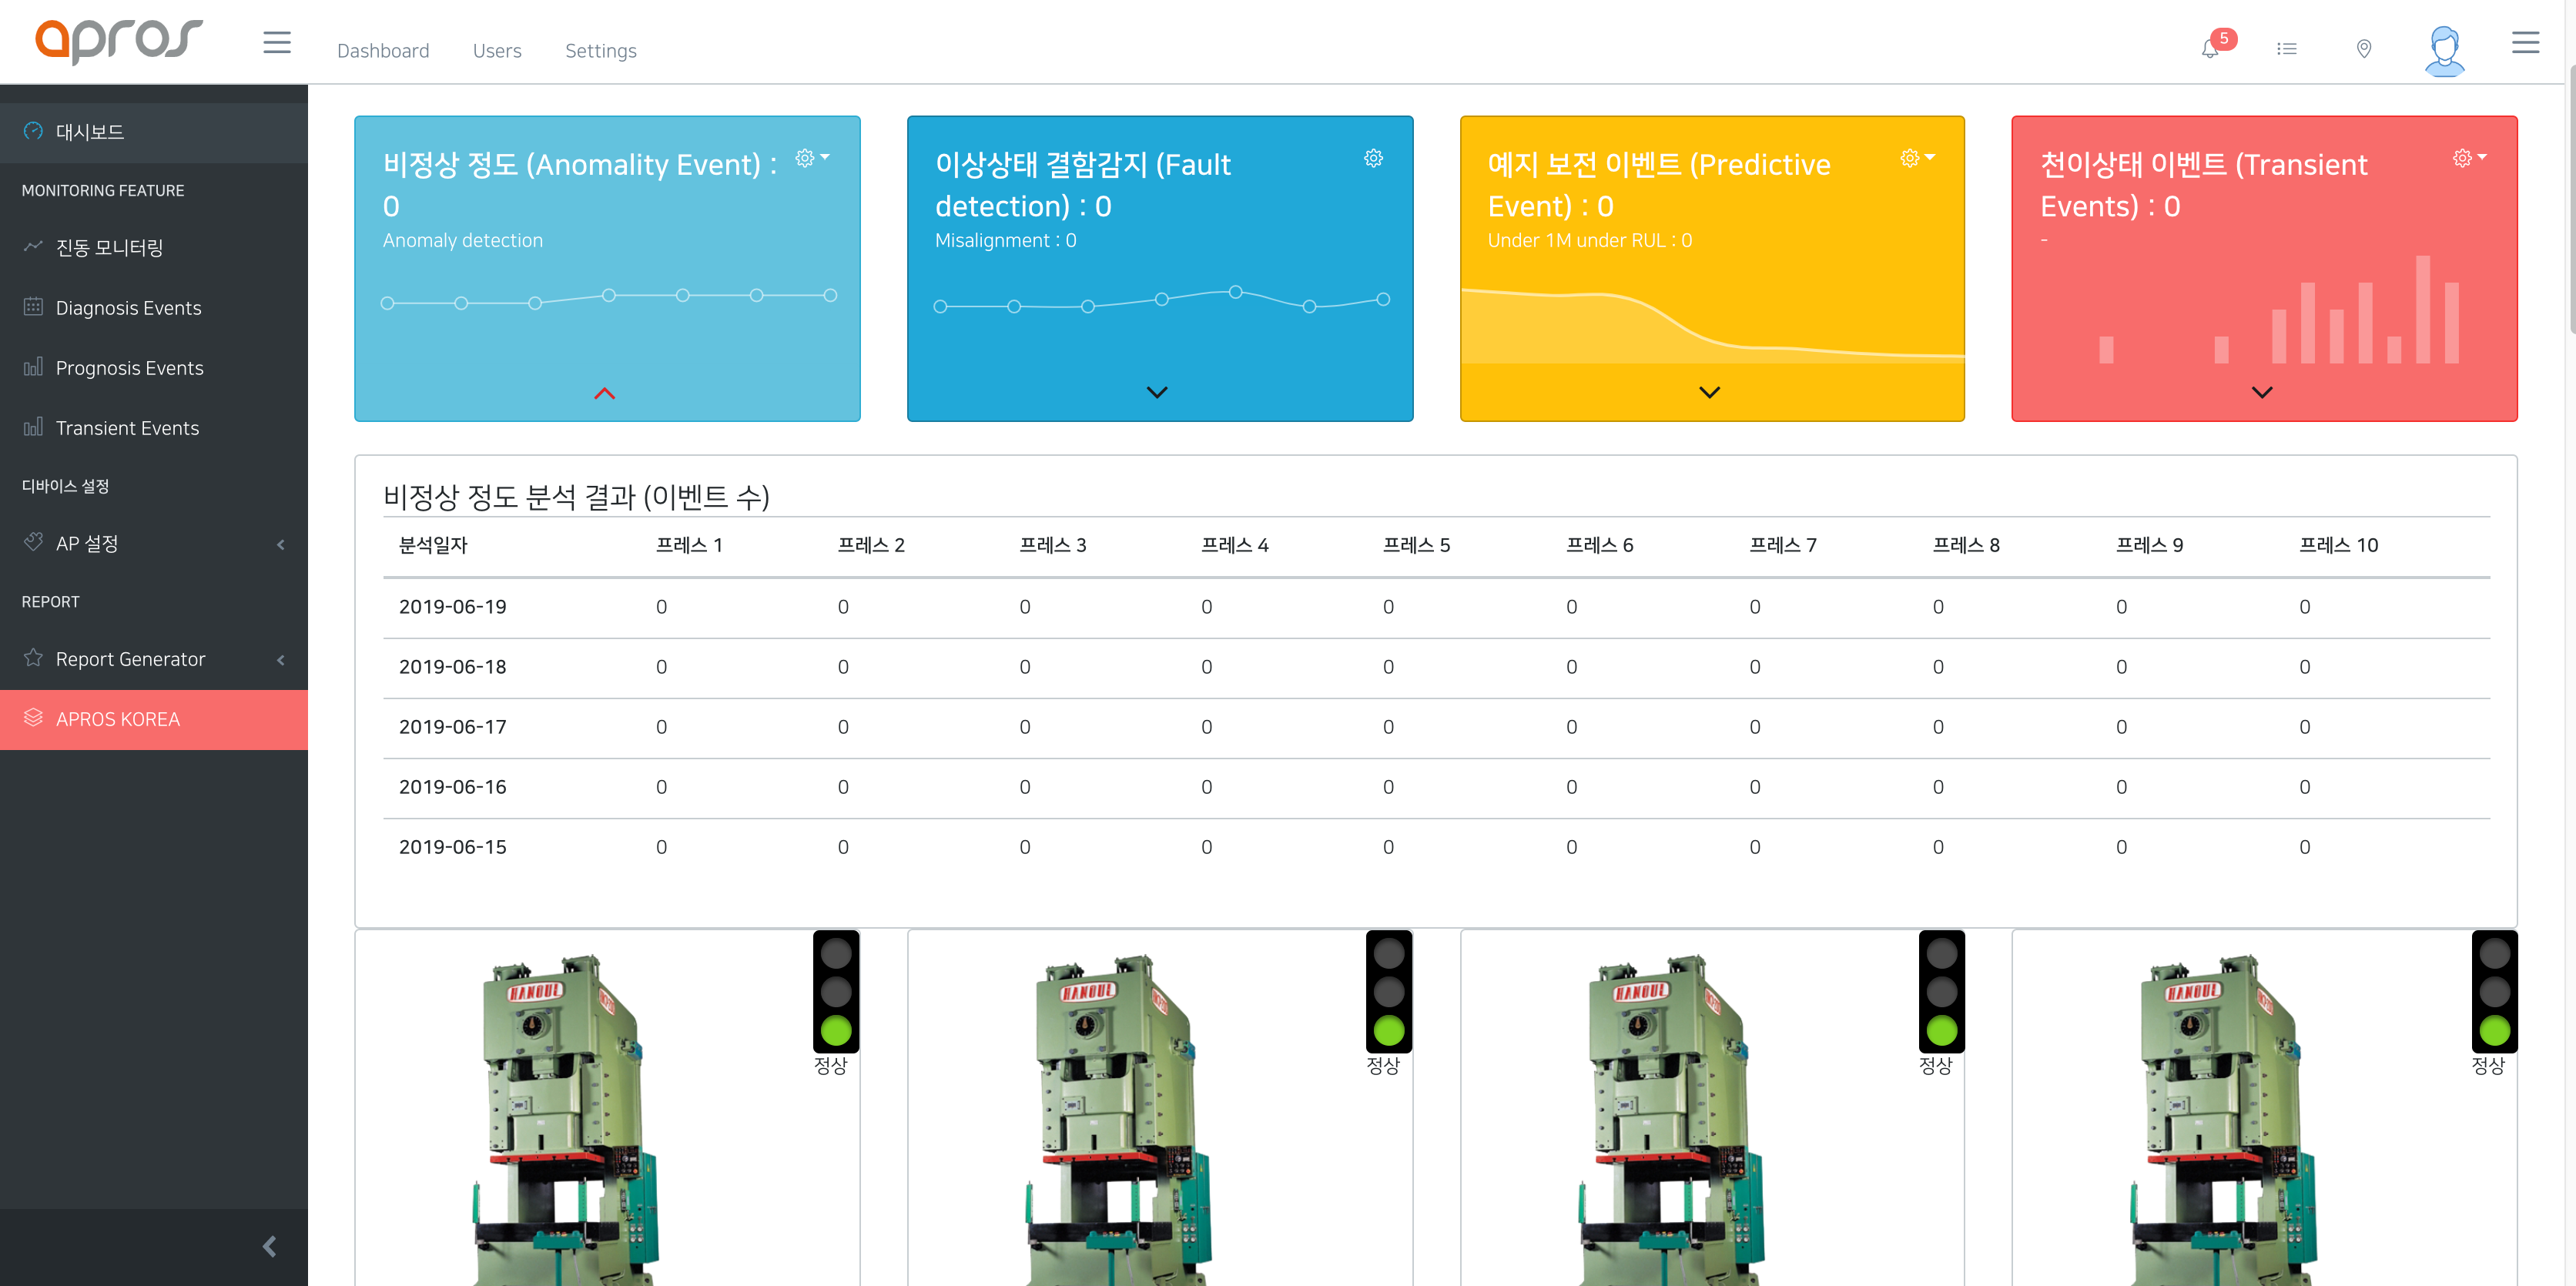
\includegraphics[width=0.5\textwidth]{images/new_dashboard_02.png}
			\caption*{Anomaly detection}
		}\qquad
		\parbox{0.5\textwidth}{
			\centering
			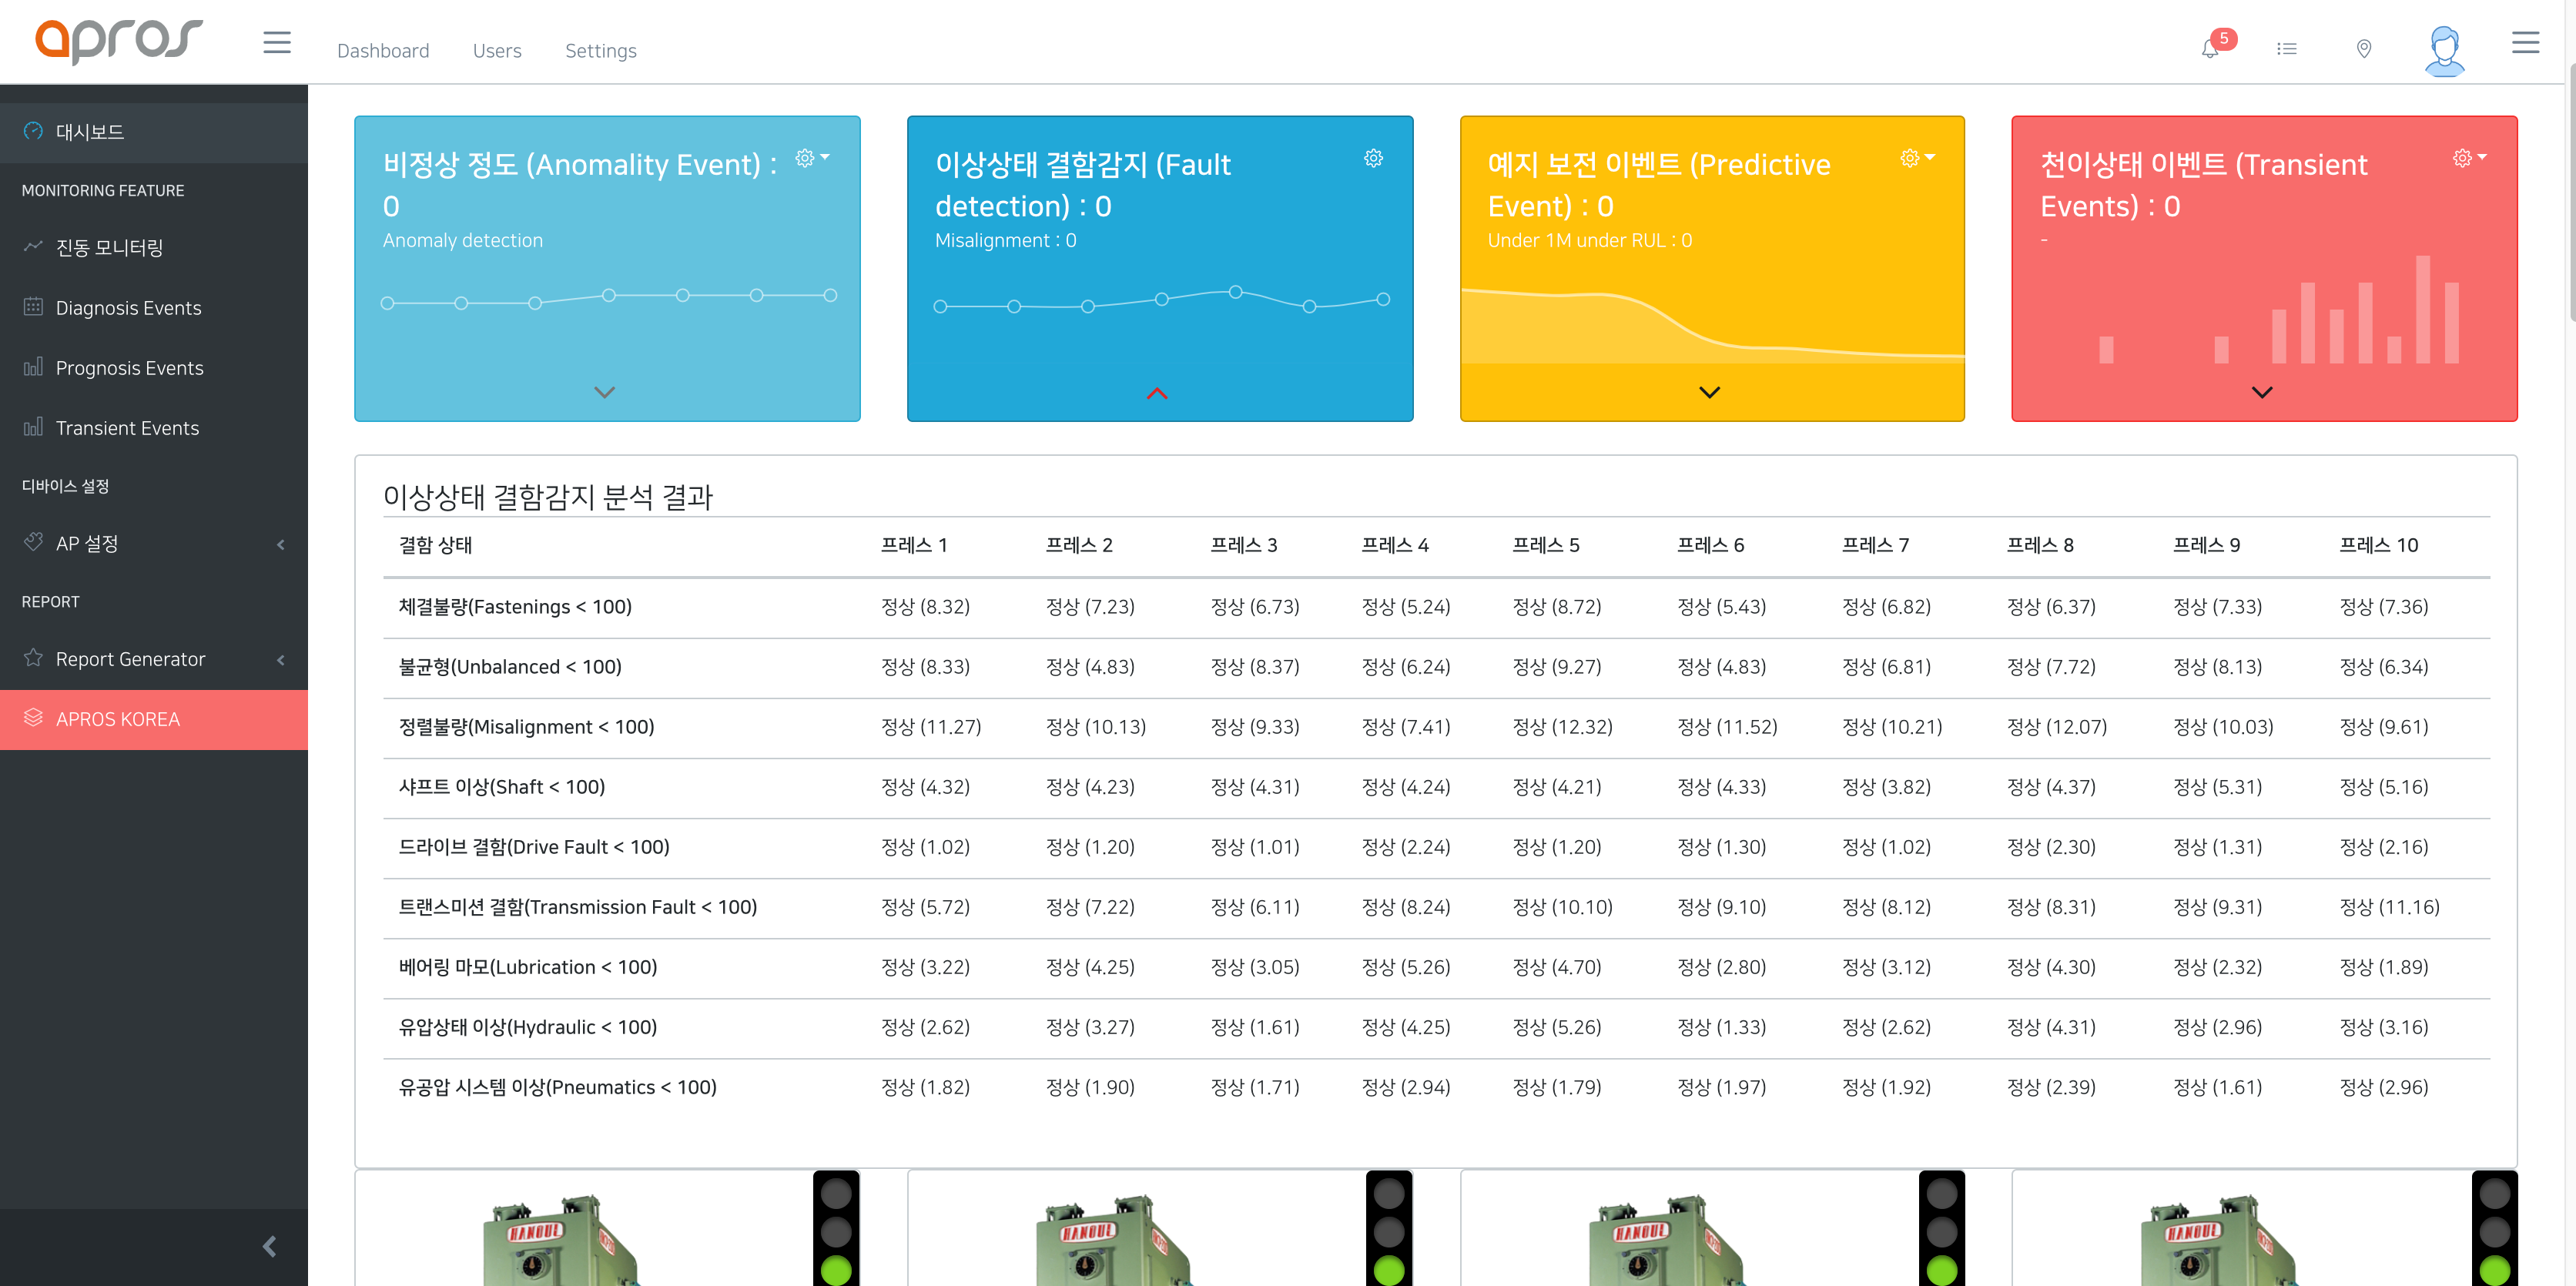
\includegraphics[width=0.5\textwidth]{images/new_dashboard_03.png}
			\caption*{Fault detection}
		}\qquad
		\parbox{0.5\textwidth}{
			\centering
			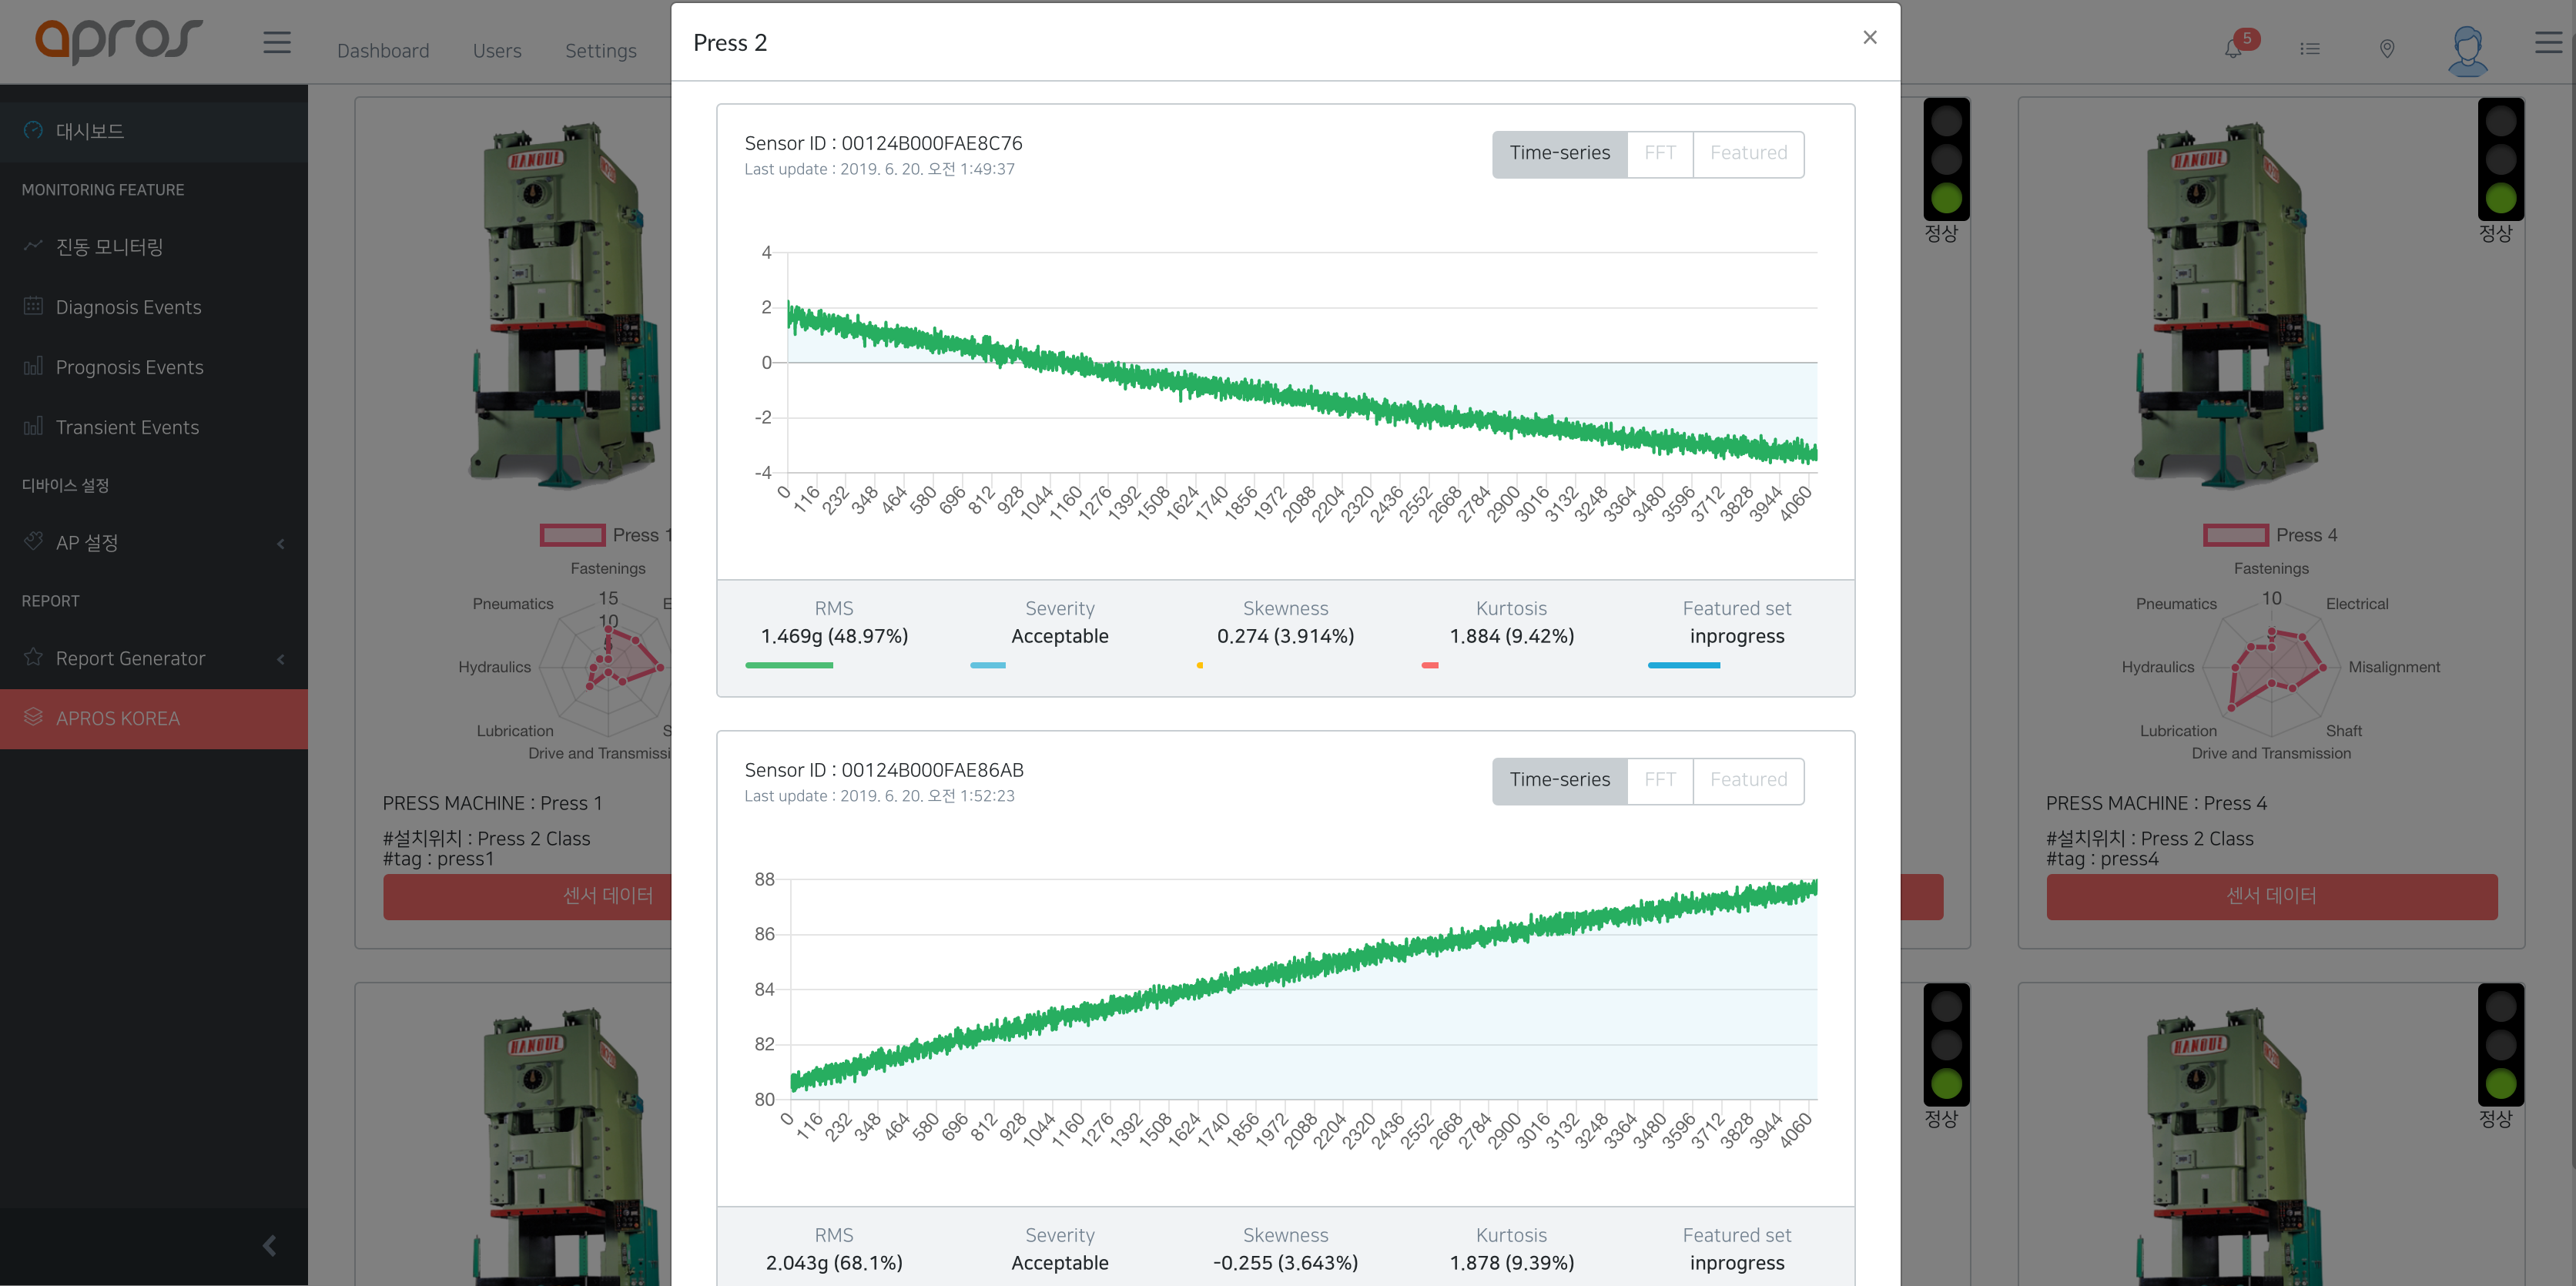
\includegraphics[width=0.5\textwidth]{images/new_dashboard_05.png}
			\caption*{데이터 조회}
		}
		\parbox{0.5\textwidth}{
			\centering
			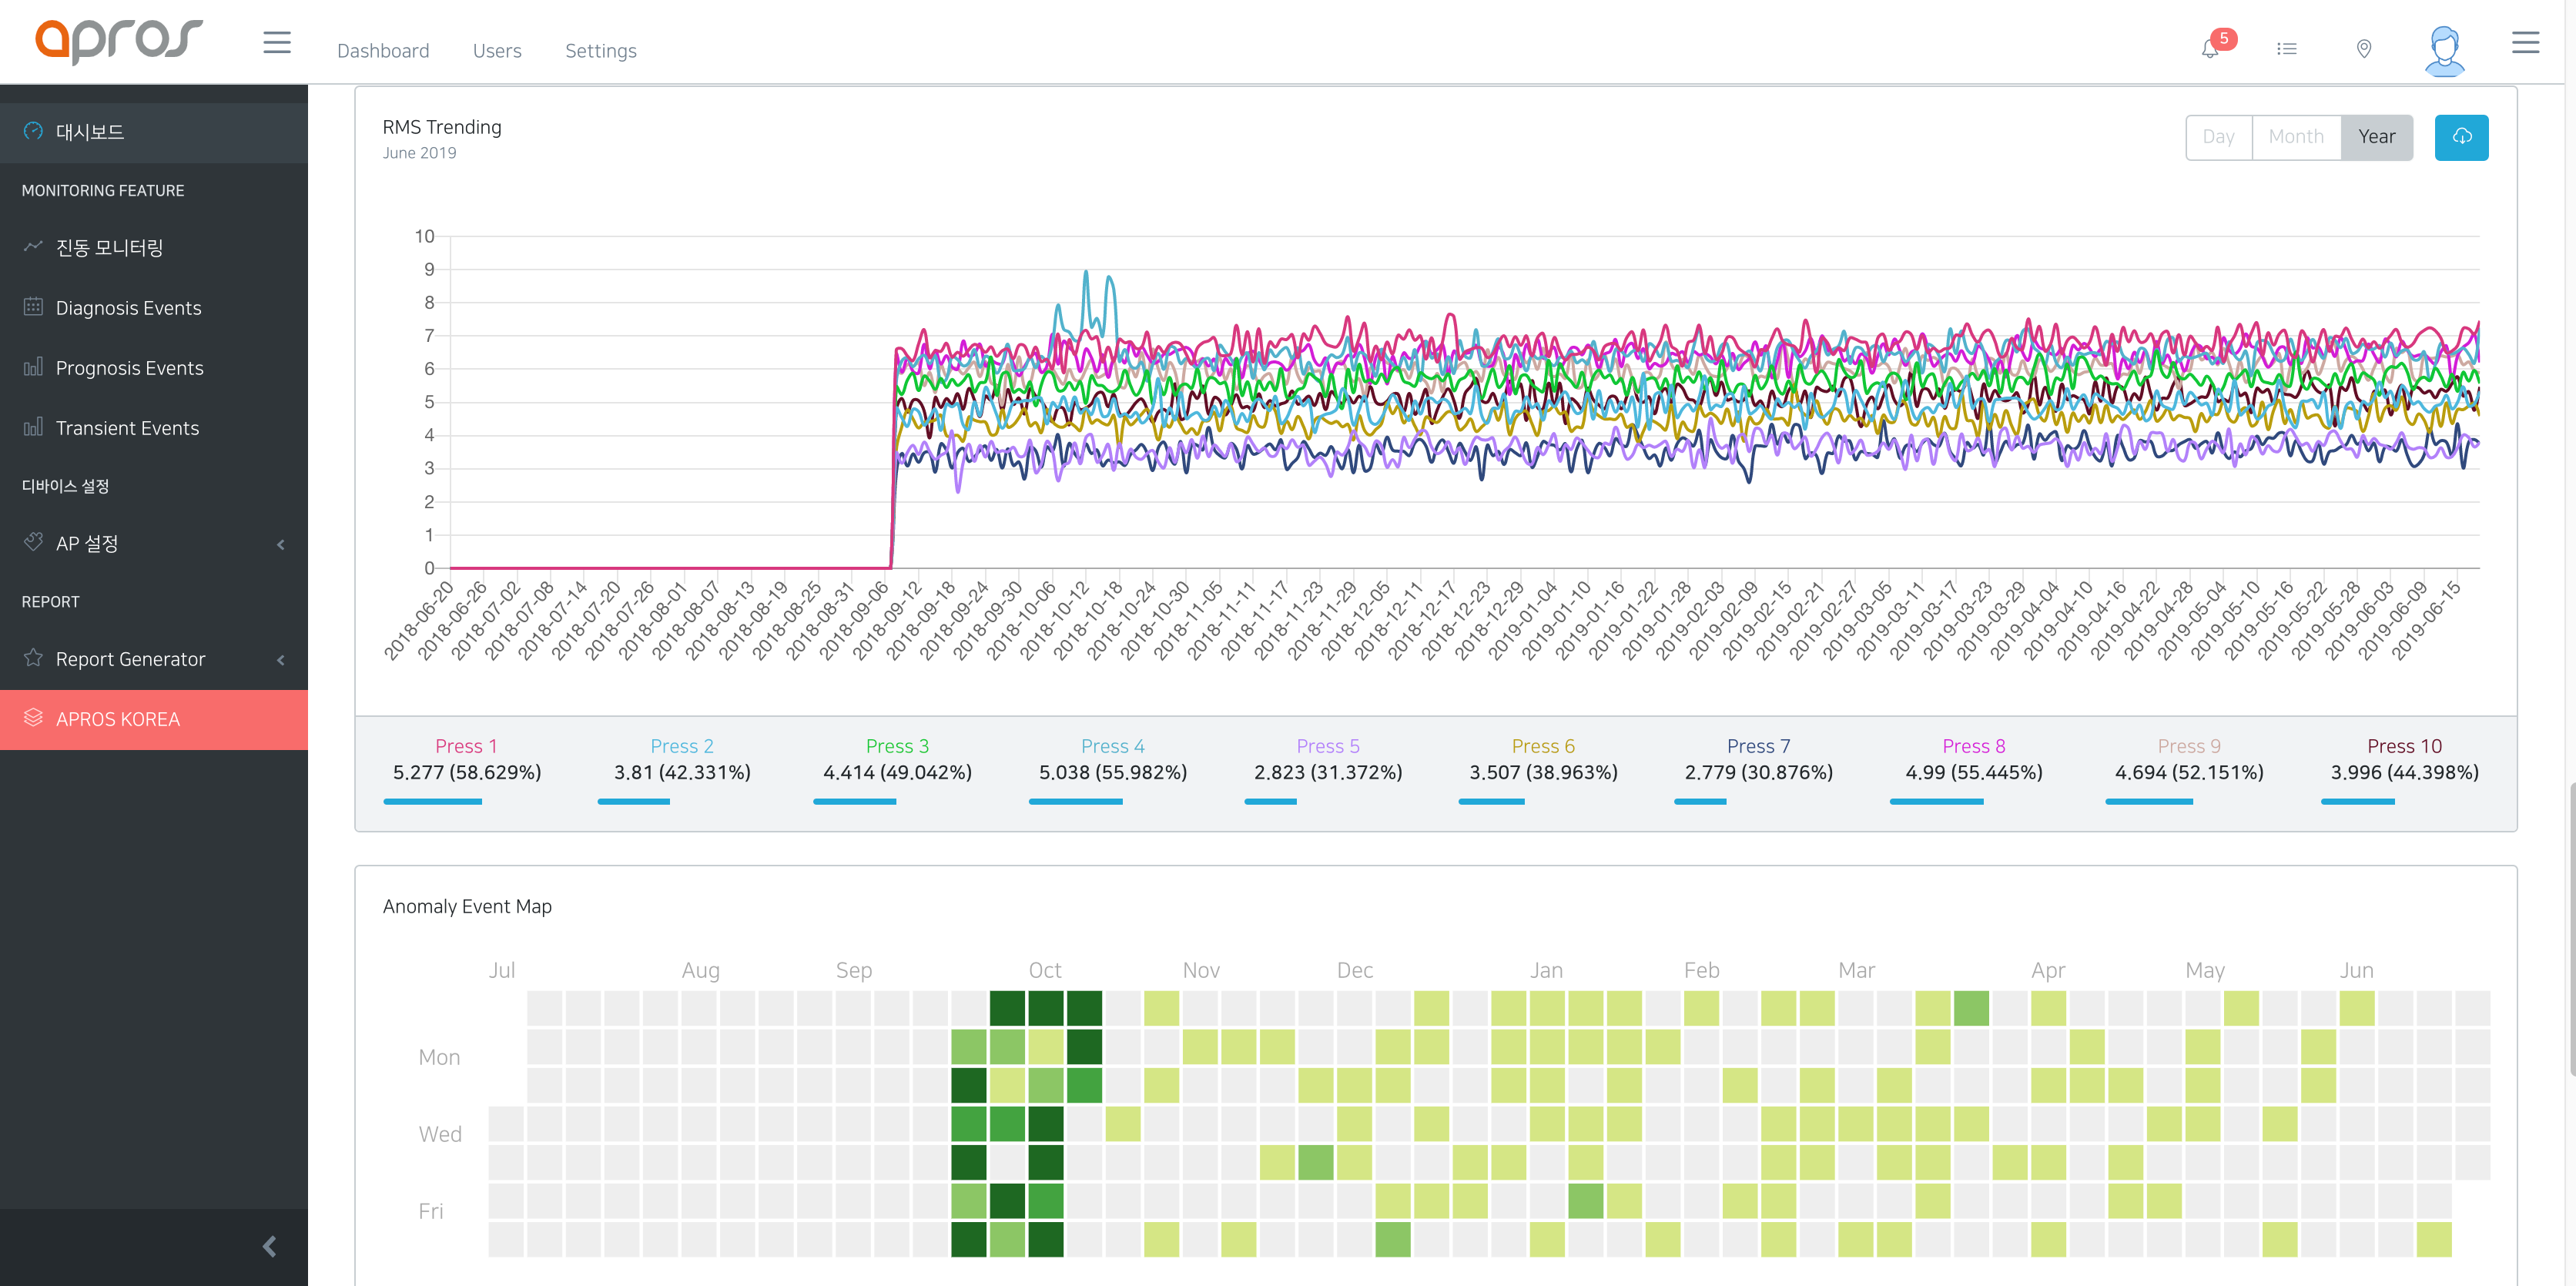
\includegraphics[width=0.5\textwidth]{images/new_dashboard_06.png}
			\caption*{Trending / Anomaly map}
		}\qquad
		\parbox{0.5\textwidth}{
			\centering
			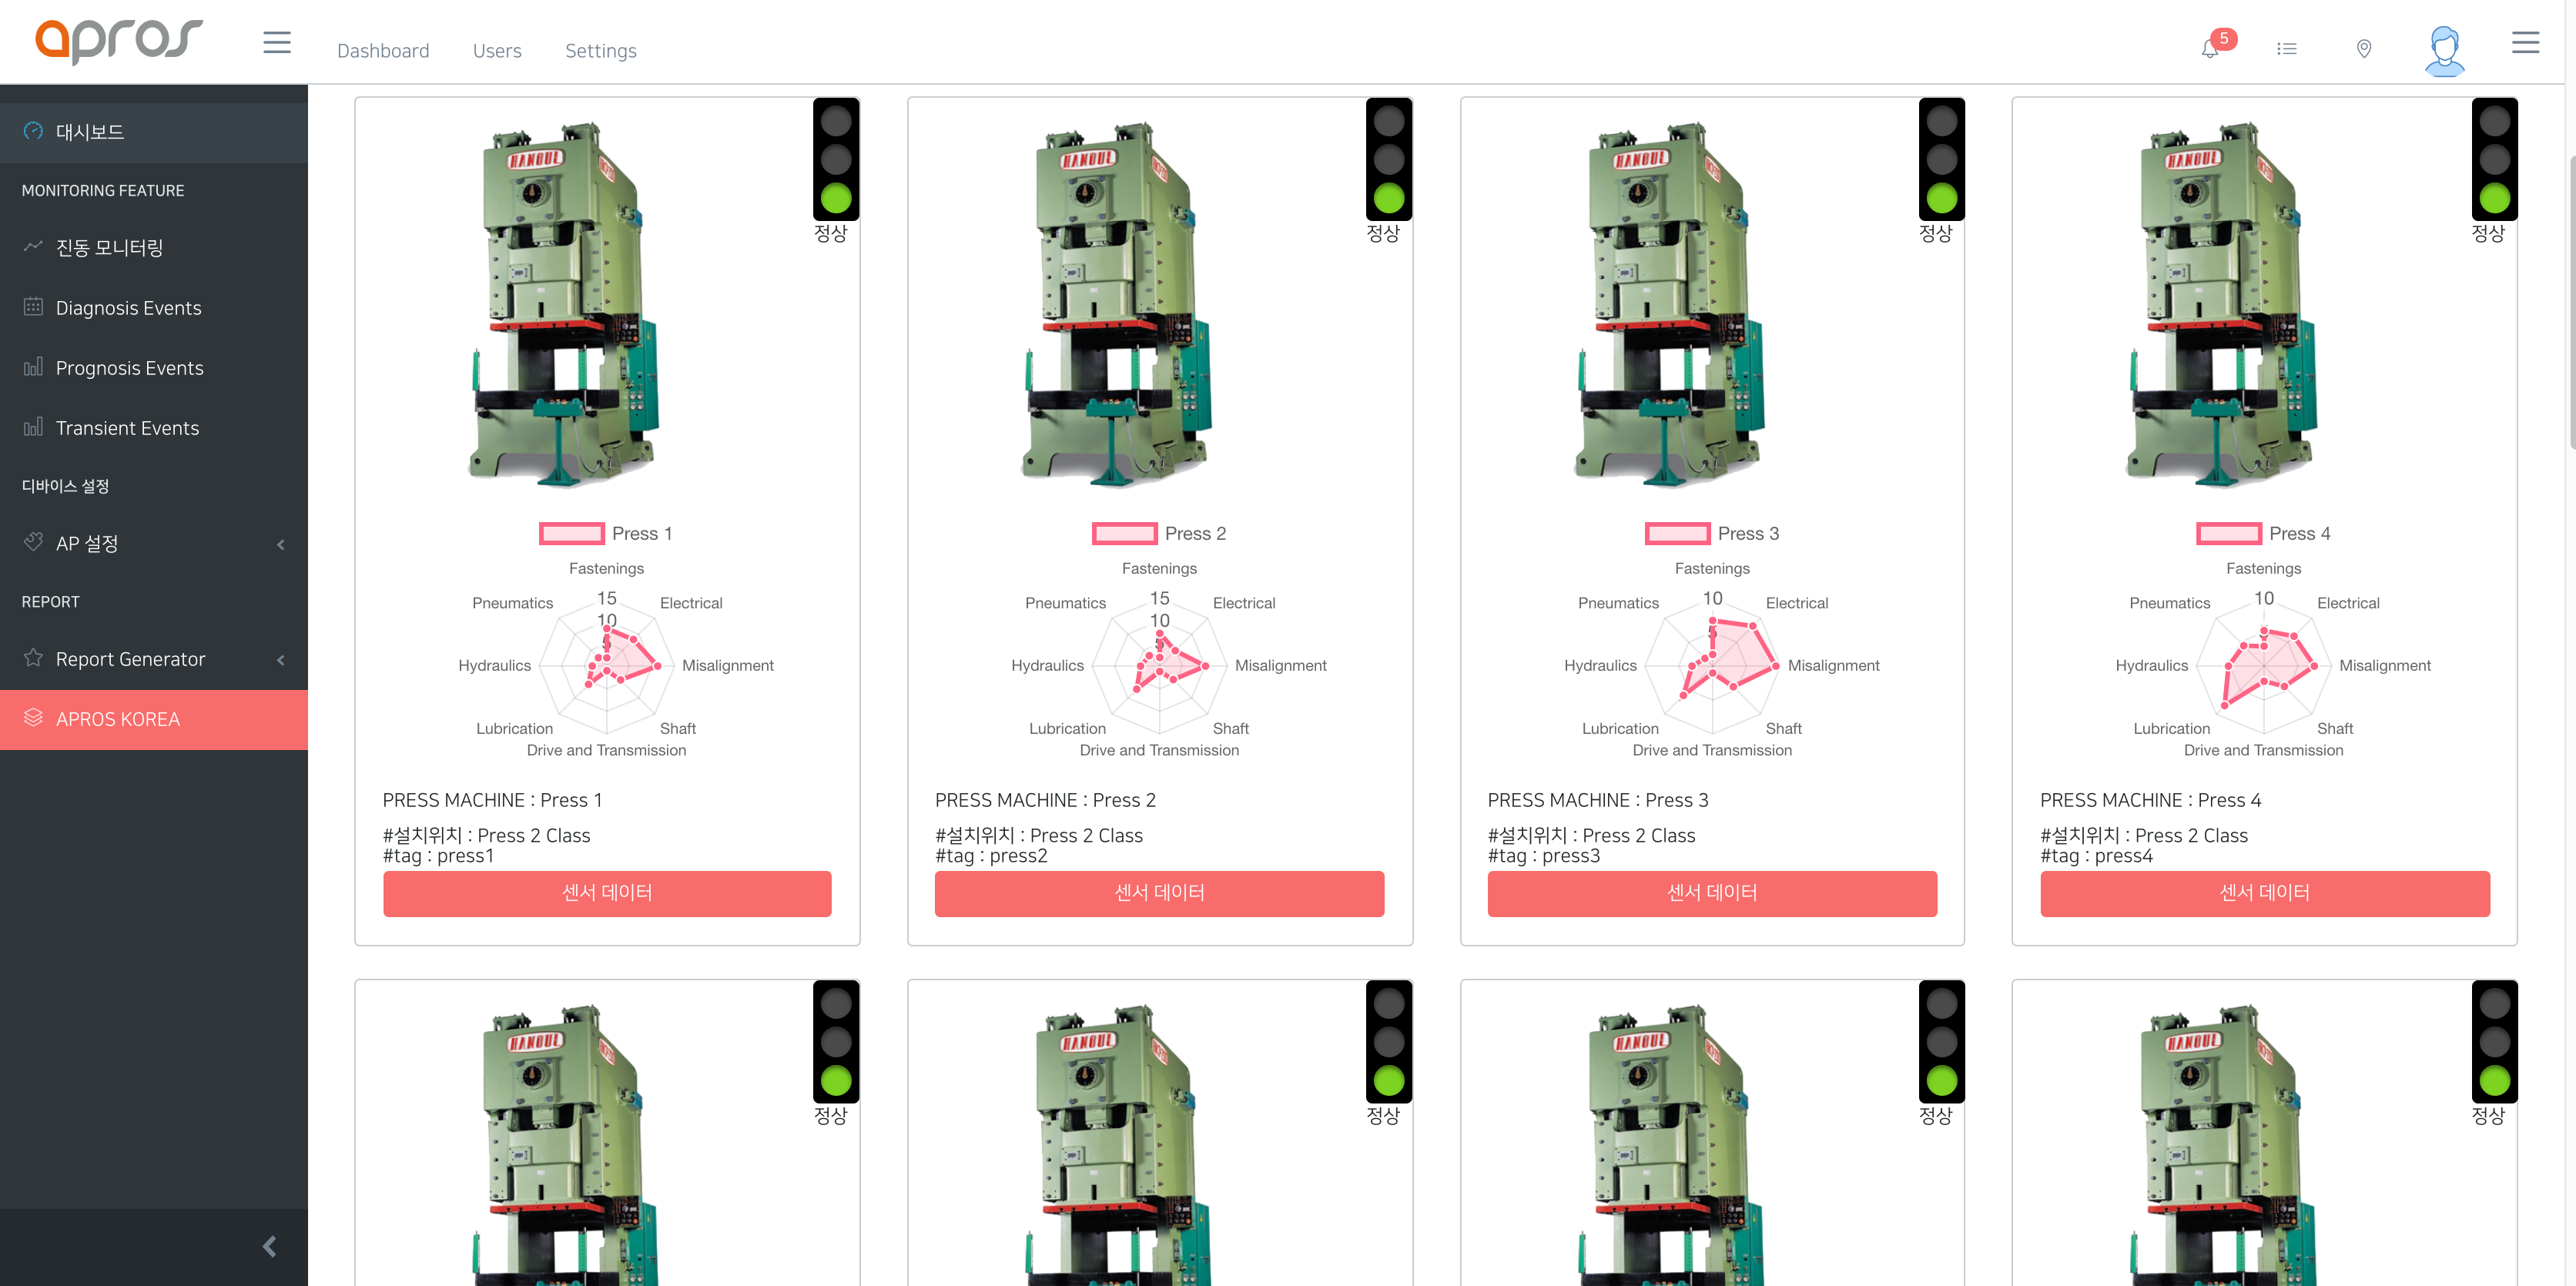
\includegraphics[width=0.5\textwidth]{images/new_dashboard_04.png}
			\caption*{설비 상태 모니터링}
		}\qquad
		\parbox{0.5\textwidth}{
			\centering
			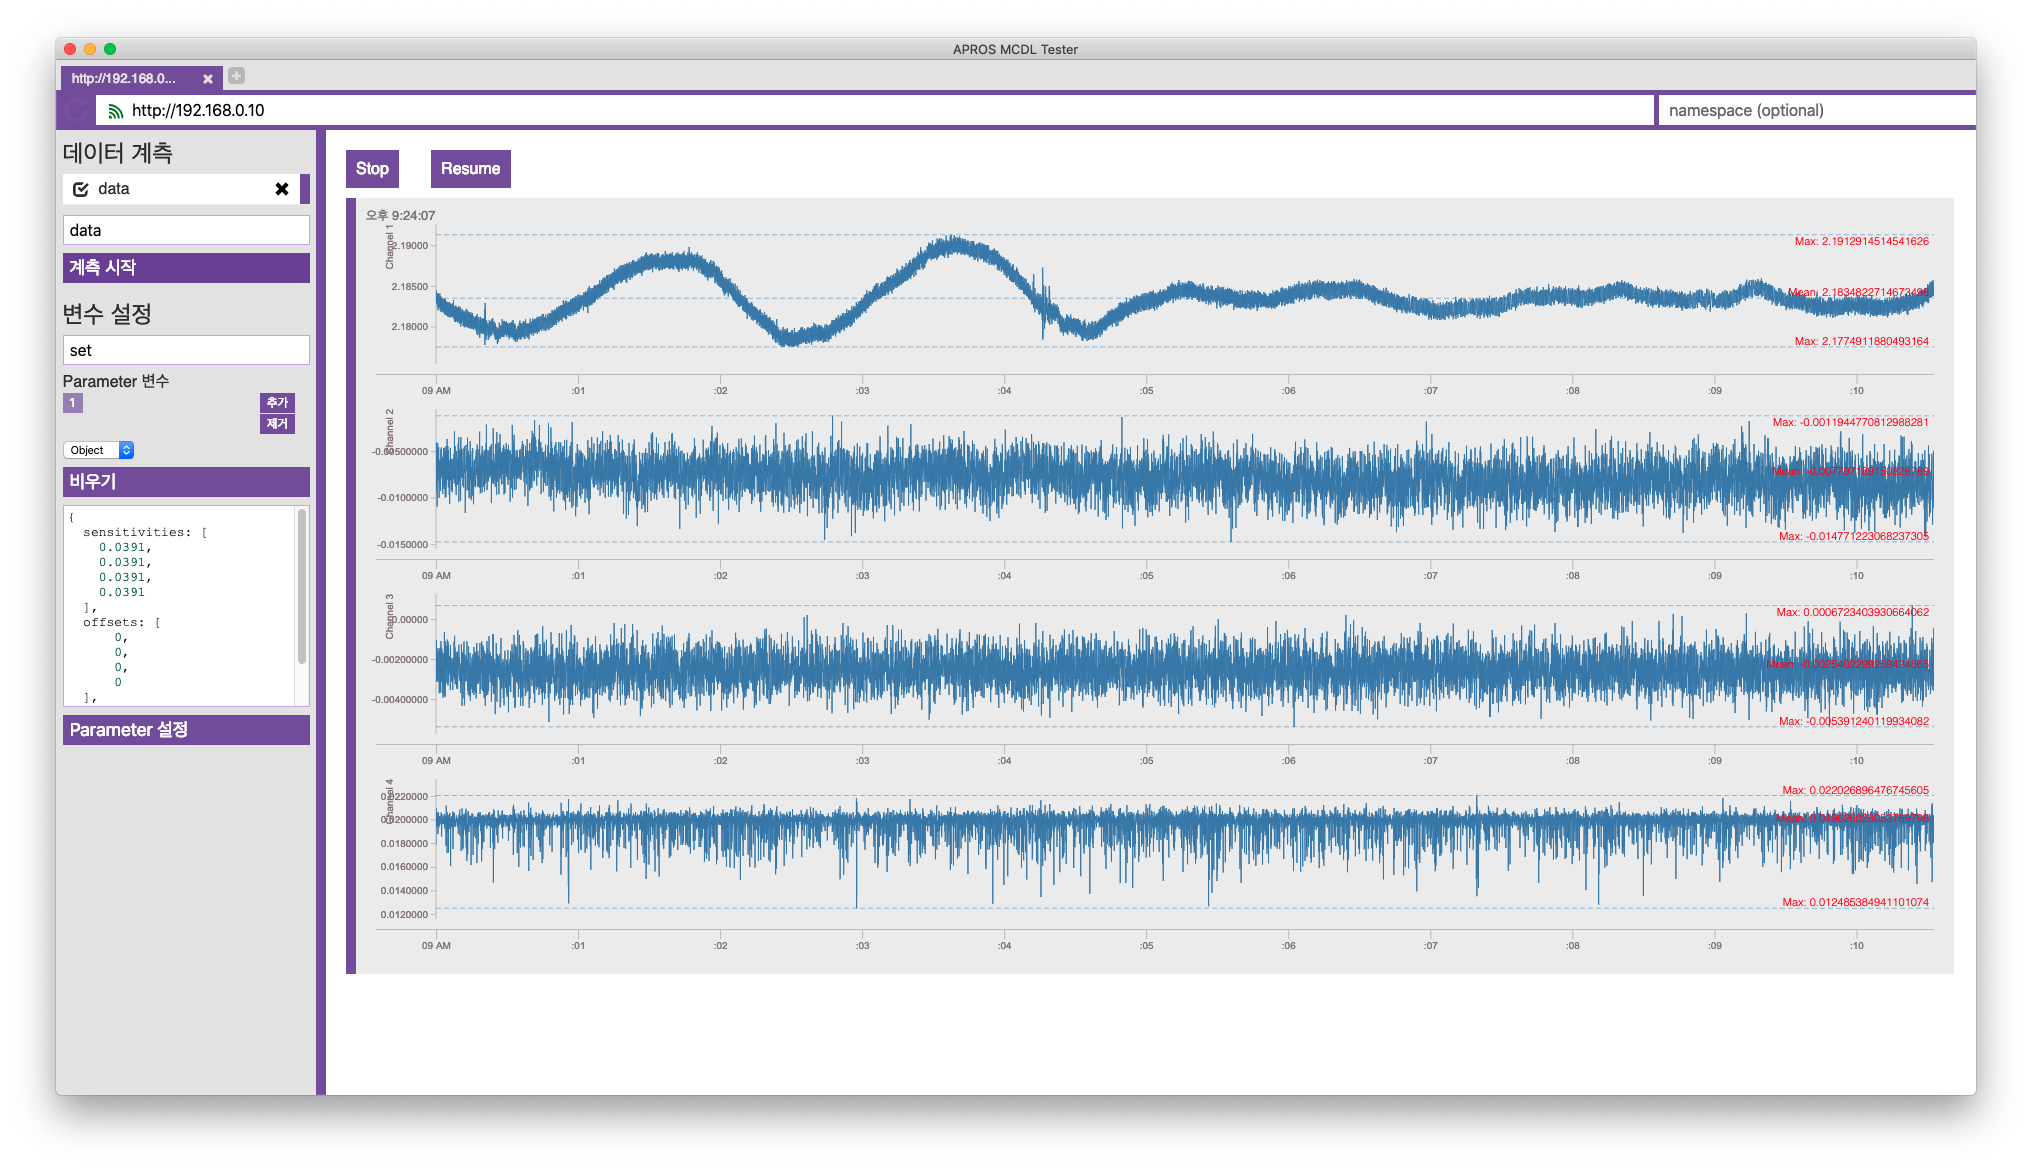
\includegraphics[width=0.5\textwidth]{images/mcdl-01.png}
			\caption*{Data logger tool (ElectronJS)}
		}
	\end{fullwidth}
\end{figure}